The electron identification procedure just described in Chapter~\ref{ch:electronid} leads nicely into the analysis portion of this thesis where those electrons are now used to look for new physics.
New physics in the form of fundamental particles that require description beyond the Standard Model and ultimately would lead to a deeper understanding of our natural world.
In this chapter we will describe just that, a search for a new fundamental particle by way of its decay into the fully visible final state of three charged leptons (a lot of which are electrons).
This fully visible final state allows for the reconstruction of the particle's invariant mass which would rise resonantly above the estimated background if seen in the data.
Figures \ref{fig:feyna} and \ref{fig:feynb} depict the the  processes of interest that give rise to the resonance via the chargino decay, \chonepm$\rightarrow$\Zboson$\ell^{\pm} \rightarrow  \ell^{\pm} \ell^{\mp} \ell^{\pm}$.
\begin{figure}[h]
  \centering
  \begin{subfigure}[b]{0.49\textwidth}
    \centering
    \includegraphics[width=1.0\textwidth]{figs/rpvthreel/fig_01b.png}
    \caption{}
    \label{fig:feyna}
  \end{subfigure}
  \hfill
  \begin{subfigure}[b]{0.49\textwidth}
    \centering
    \includegraphics[width=1.00\textwidth]{figs/rpvthreel/fig_01b.png}
    \caption{}
    \label{fig:feynb}
  \end{subfigure}
  \caption[Diagrams of (a) \CCsignal and \CNsignal (b) production with at least one \chonepm$\rightarrow$\Zboson $\ell \rightarrow \ell\ell\ell$ decay.]{Diagrams of (a) \CCsignal and \CCsignal (b) production with at least one \chonepm$\rightarrow$\Zboson$\ell\rightarrow\ell\ell\ell$ decay.
  The R-parity-violating coupling $\epsilon_{i}$ allows prompt \chonepm decays into \Zboson$\ell$, \Hboson$\ell$ or \Wboson$\nu$ and prompt \none decays into \Wboson$\ell$, \Zboson$\nu$, or \Hboson$\nu$ ~\cite{ATLAS:2020uer}.}
  \label{fig:feyn}
\end{figure}

\subsection{Phenomenological Motivation}
As alluded to in Chapter \ref{ch:theory} the theoretical framework that is used to drive this search is the \BL MSSM. 
Where in Chapter \ref{ch:theory}, the \BL MSSM was strongly motivated, we now motivate a group of experimental signatures that are likely to be seen at the ATLAS experiment in the context of this model.
Strong theoretical motivation comes from an extensive study involving the statistical scanning over all dimensionful parameters of the soft SUSY breaking terms \cite{Dumitru:2018jyb}.
A statistical analysis involving 100 million independent trials of these parameters is performed.
Where the SUSY breaking scale is restricted to 1.5~\tev or below in order to ensure that the LHC would have sufficient energy to be able to produce the LSP.
For the 100 million sets of randomly scattered initial conditions, it was found that 4,351,809 break \BL symmetry with the $Z'_{B-L}$ mass above the current lower bound of $Z'_{B-L}$ = 4.1~\tev.
\begin{figure}
    \centering
    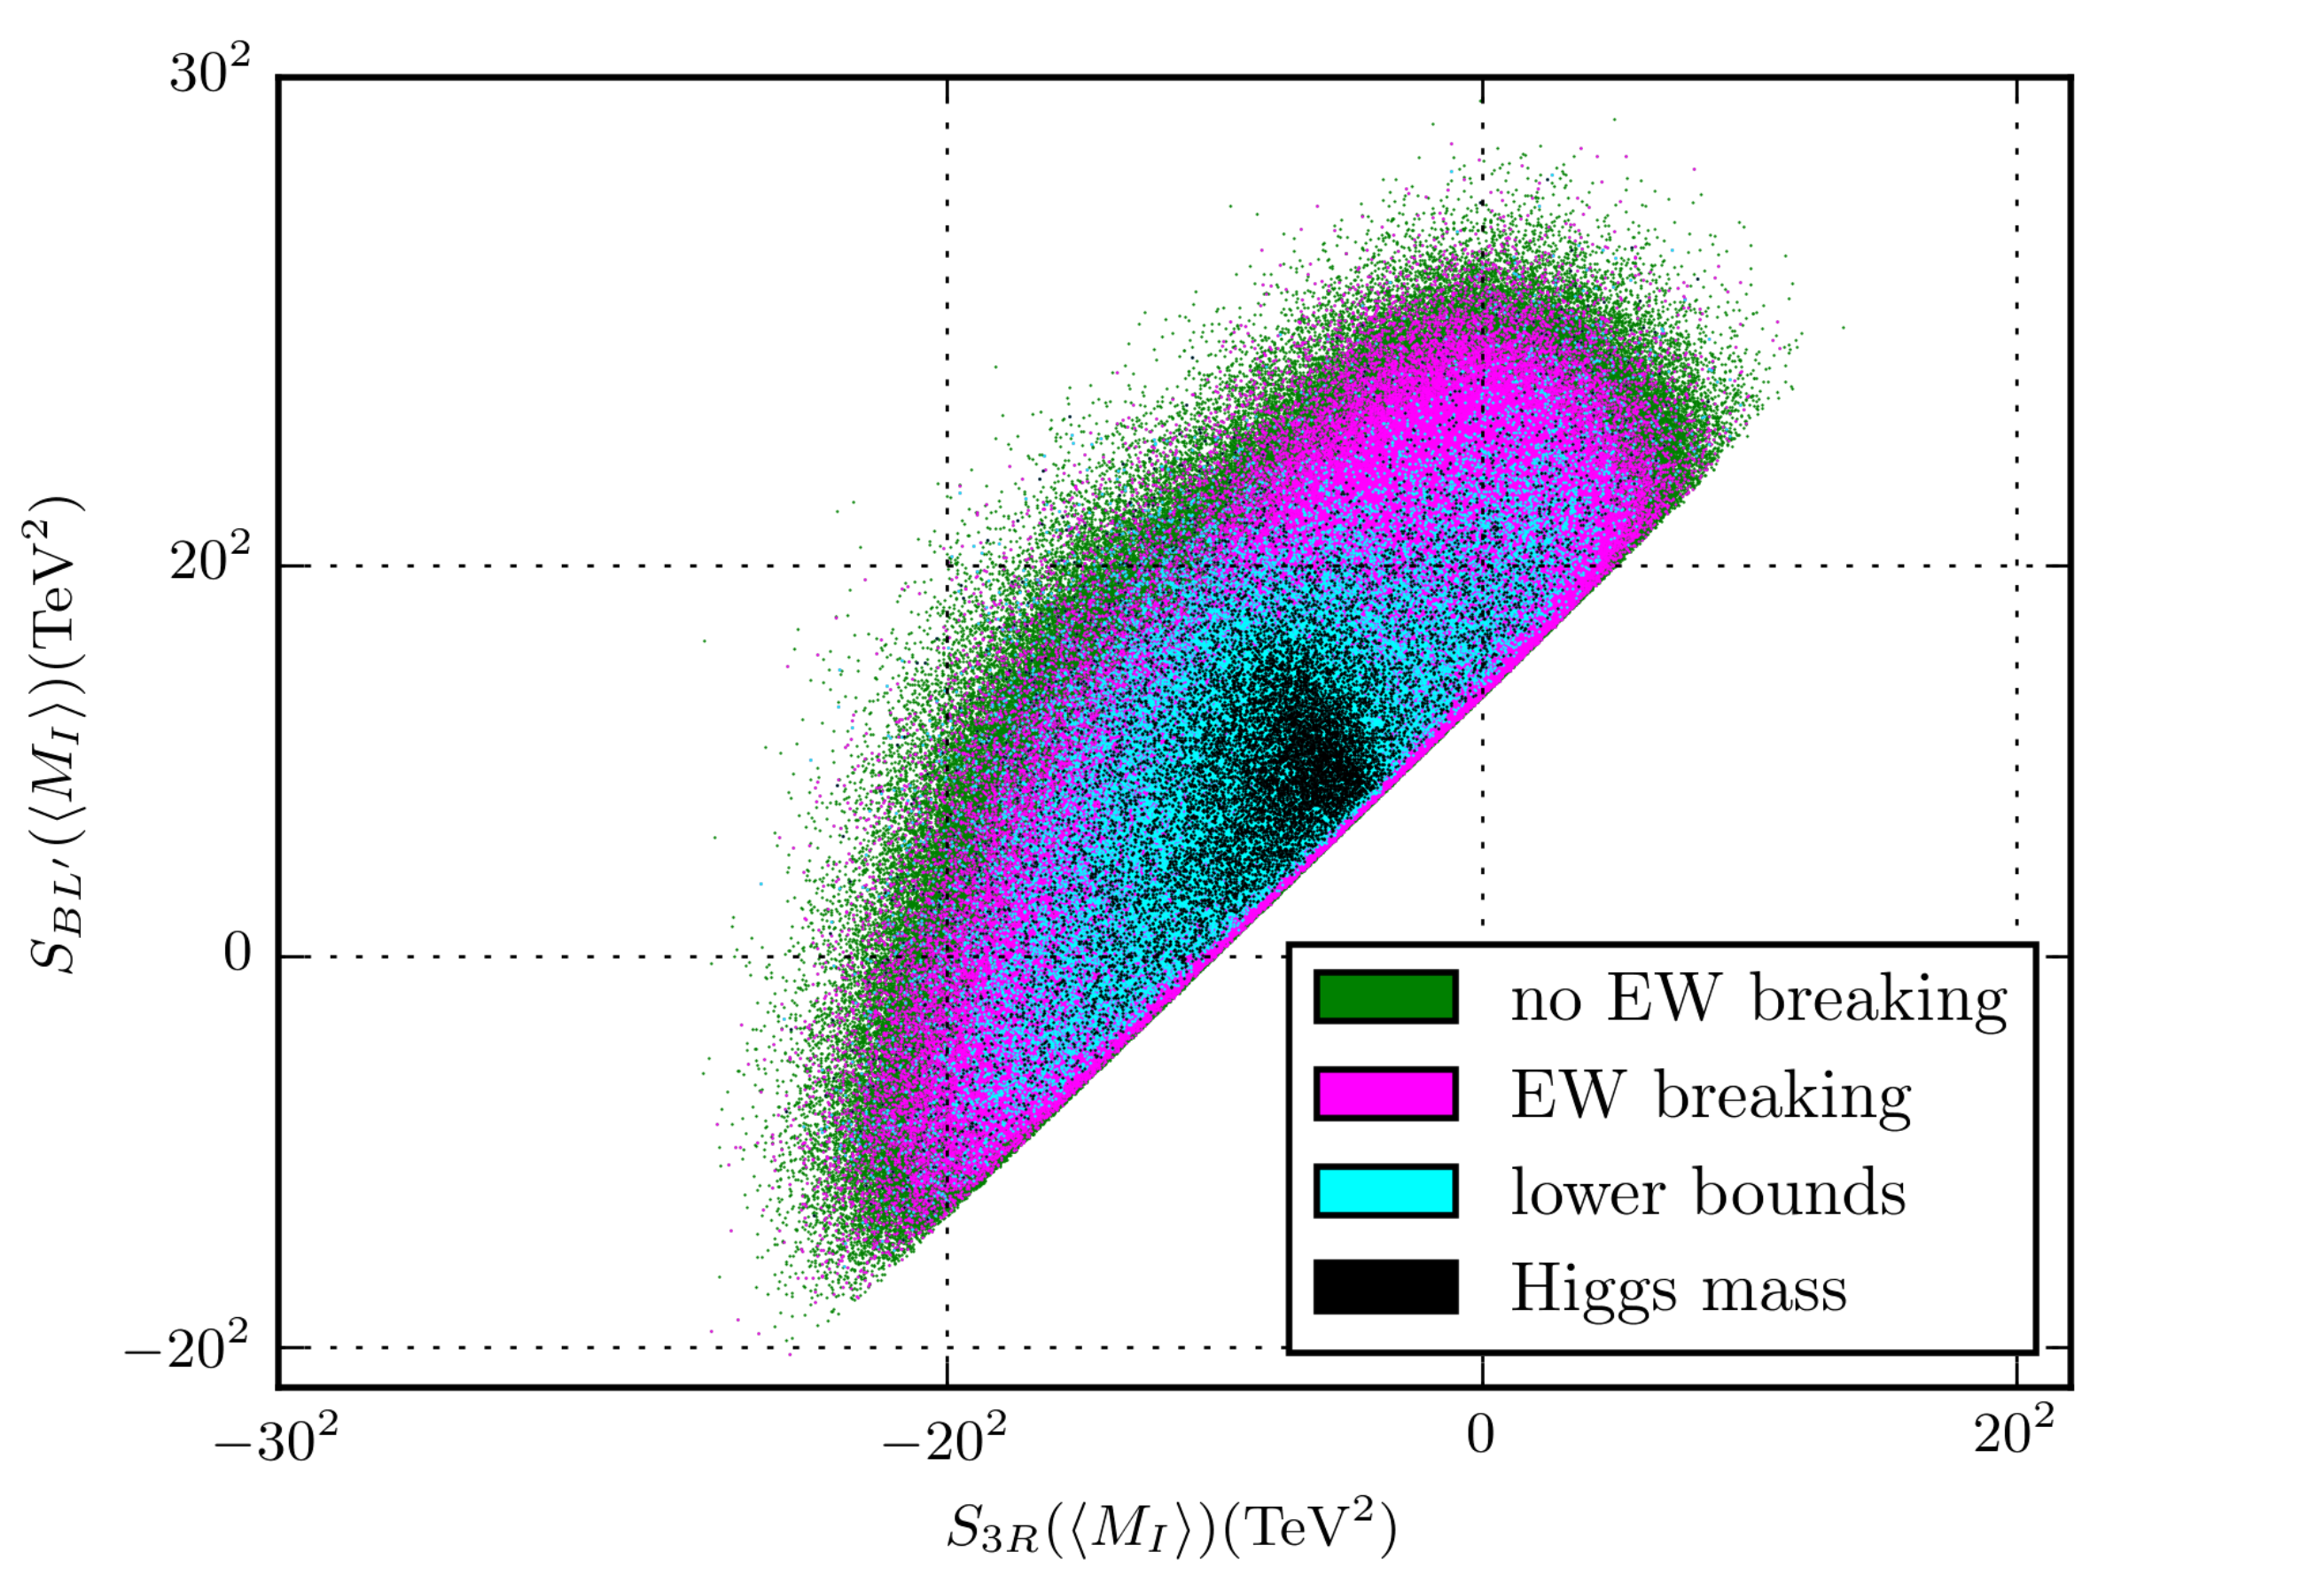
\includegraphics[width=0.95\textwidth]{figs/rpvthreel/statthrows.png}
    \caption[Plot of initial 100 million statistical trials of SUSY parameters and the subsequent filtering out of said points that do not satisfy necessary physical bounds.]{Plot of the 100 million initial data points for the analysis.
    The 4,351,809 green points lead to appropriate breaking of the \BL symmetry.
    The 3,142,657 purple points also break the EW symmetry with the correct vector boson masses.
    The cyan points correspond to 342,236 also satisfy all lower bounds on the sparticle masses.
    Finally, as a subset of these 342,236 initial points, there are 67,576 valid black points which lead to the experimentally measured value of the Higgs boson mass \cite{Dumitru:2018jyb}.}
    \label{fig:statthrows}
\end{figure}
\begin{figure}
    \centering
    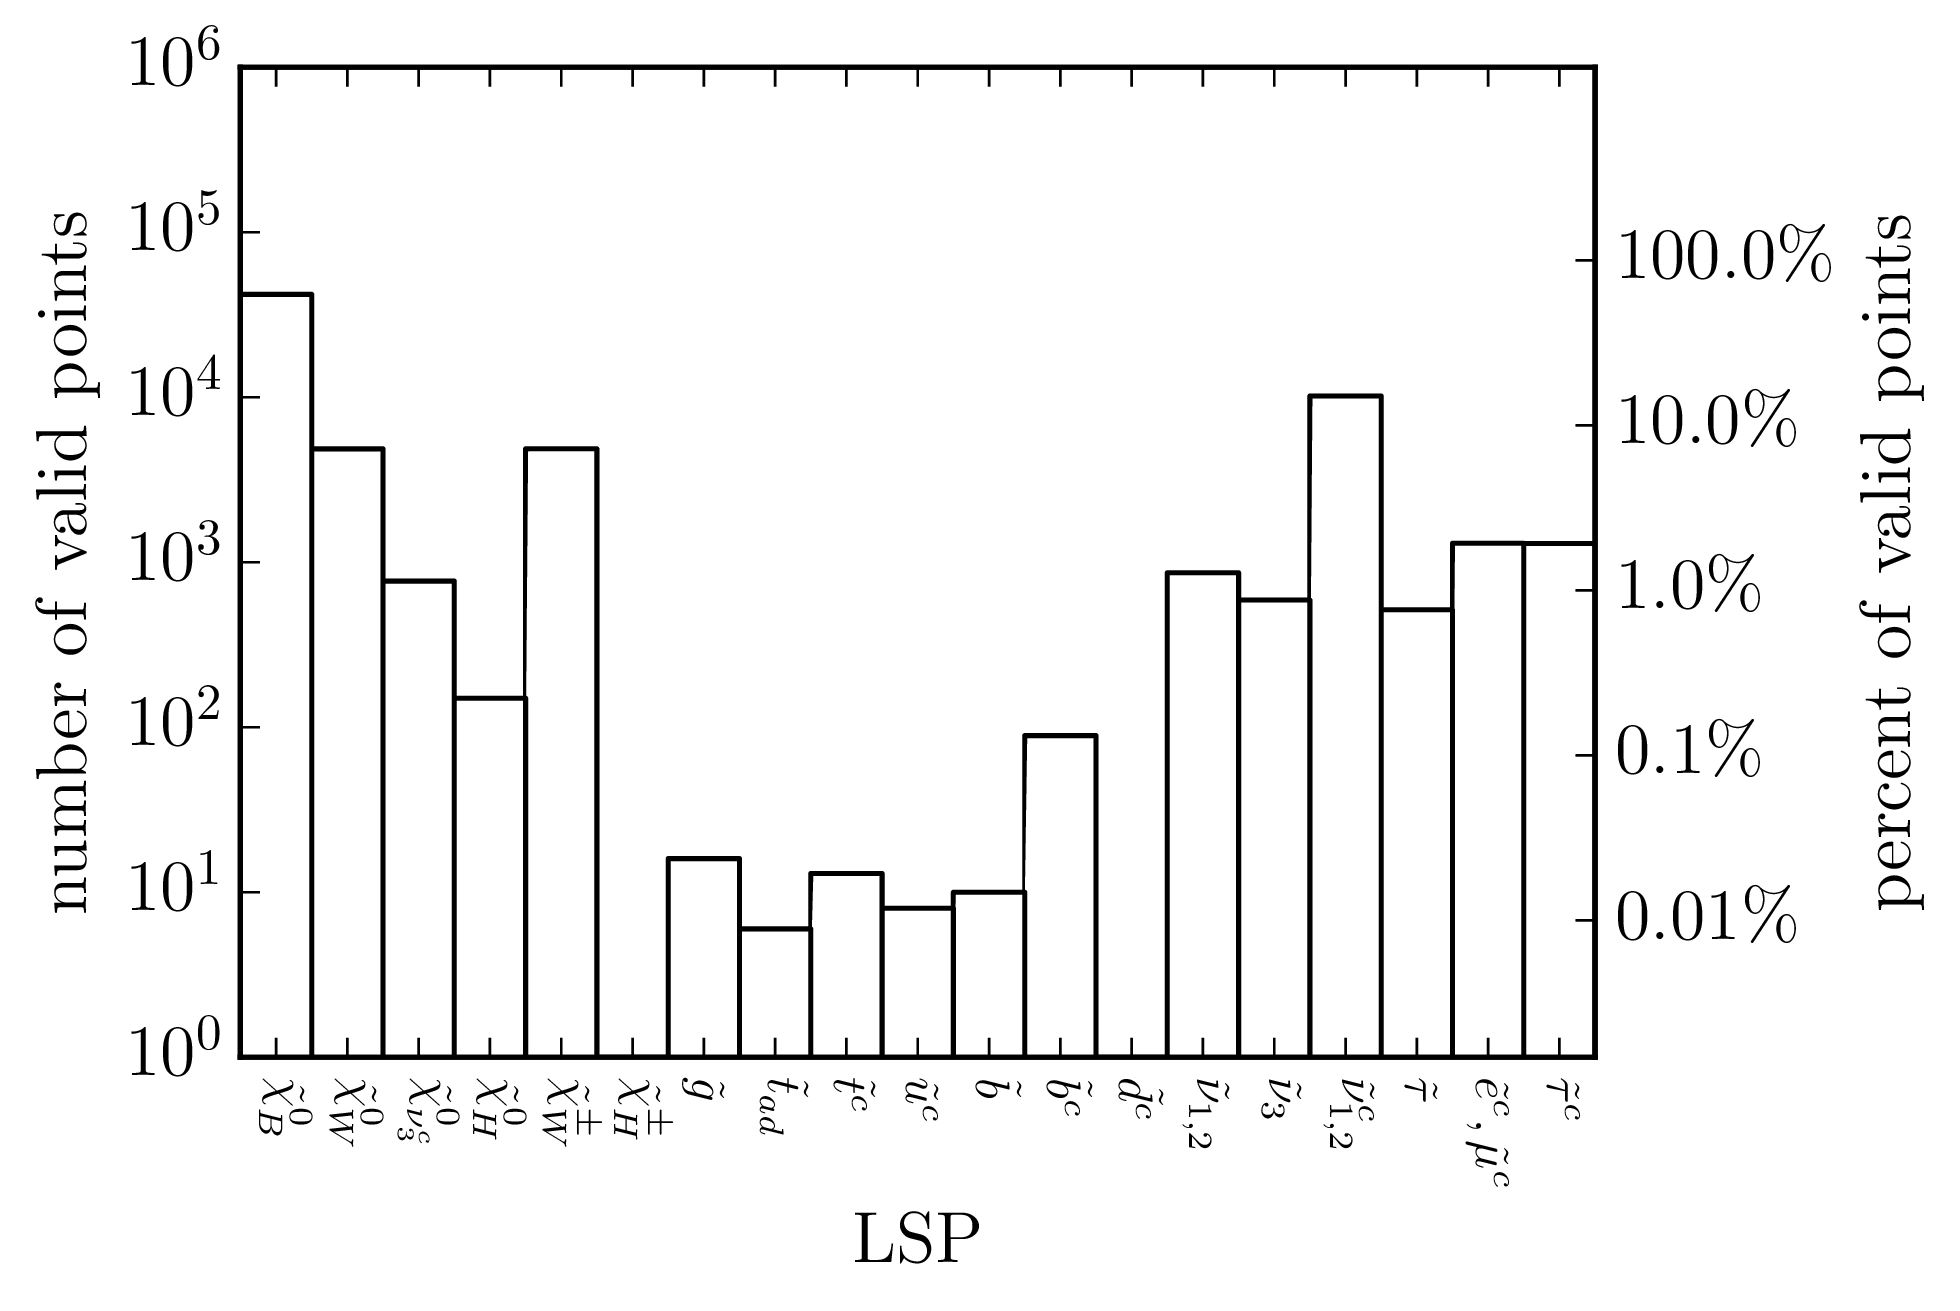
\includegraphics[width=0.95\textwidth]{figs/rpvthreel/LSPprobability.png}
    \caption[histogram of the LSPs for the valid points of the statistical analysis]{A histogram of the identity of the LSP for the 67,576 valid points.
    The left scale shows the number of valid points and the right scale shows the percent of valid points.
    Sparticles which did not appear as LSPs are omitted~\cite{Dumitru:2018nct}.}
    \label{fig:LSPprob}
\end{figure}
\begin{figure}
    \centering
    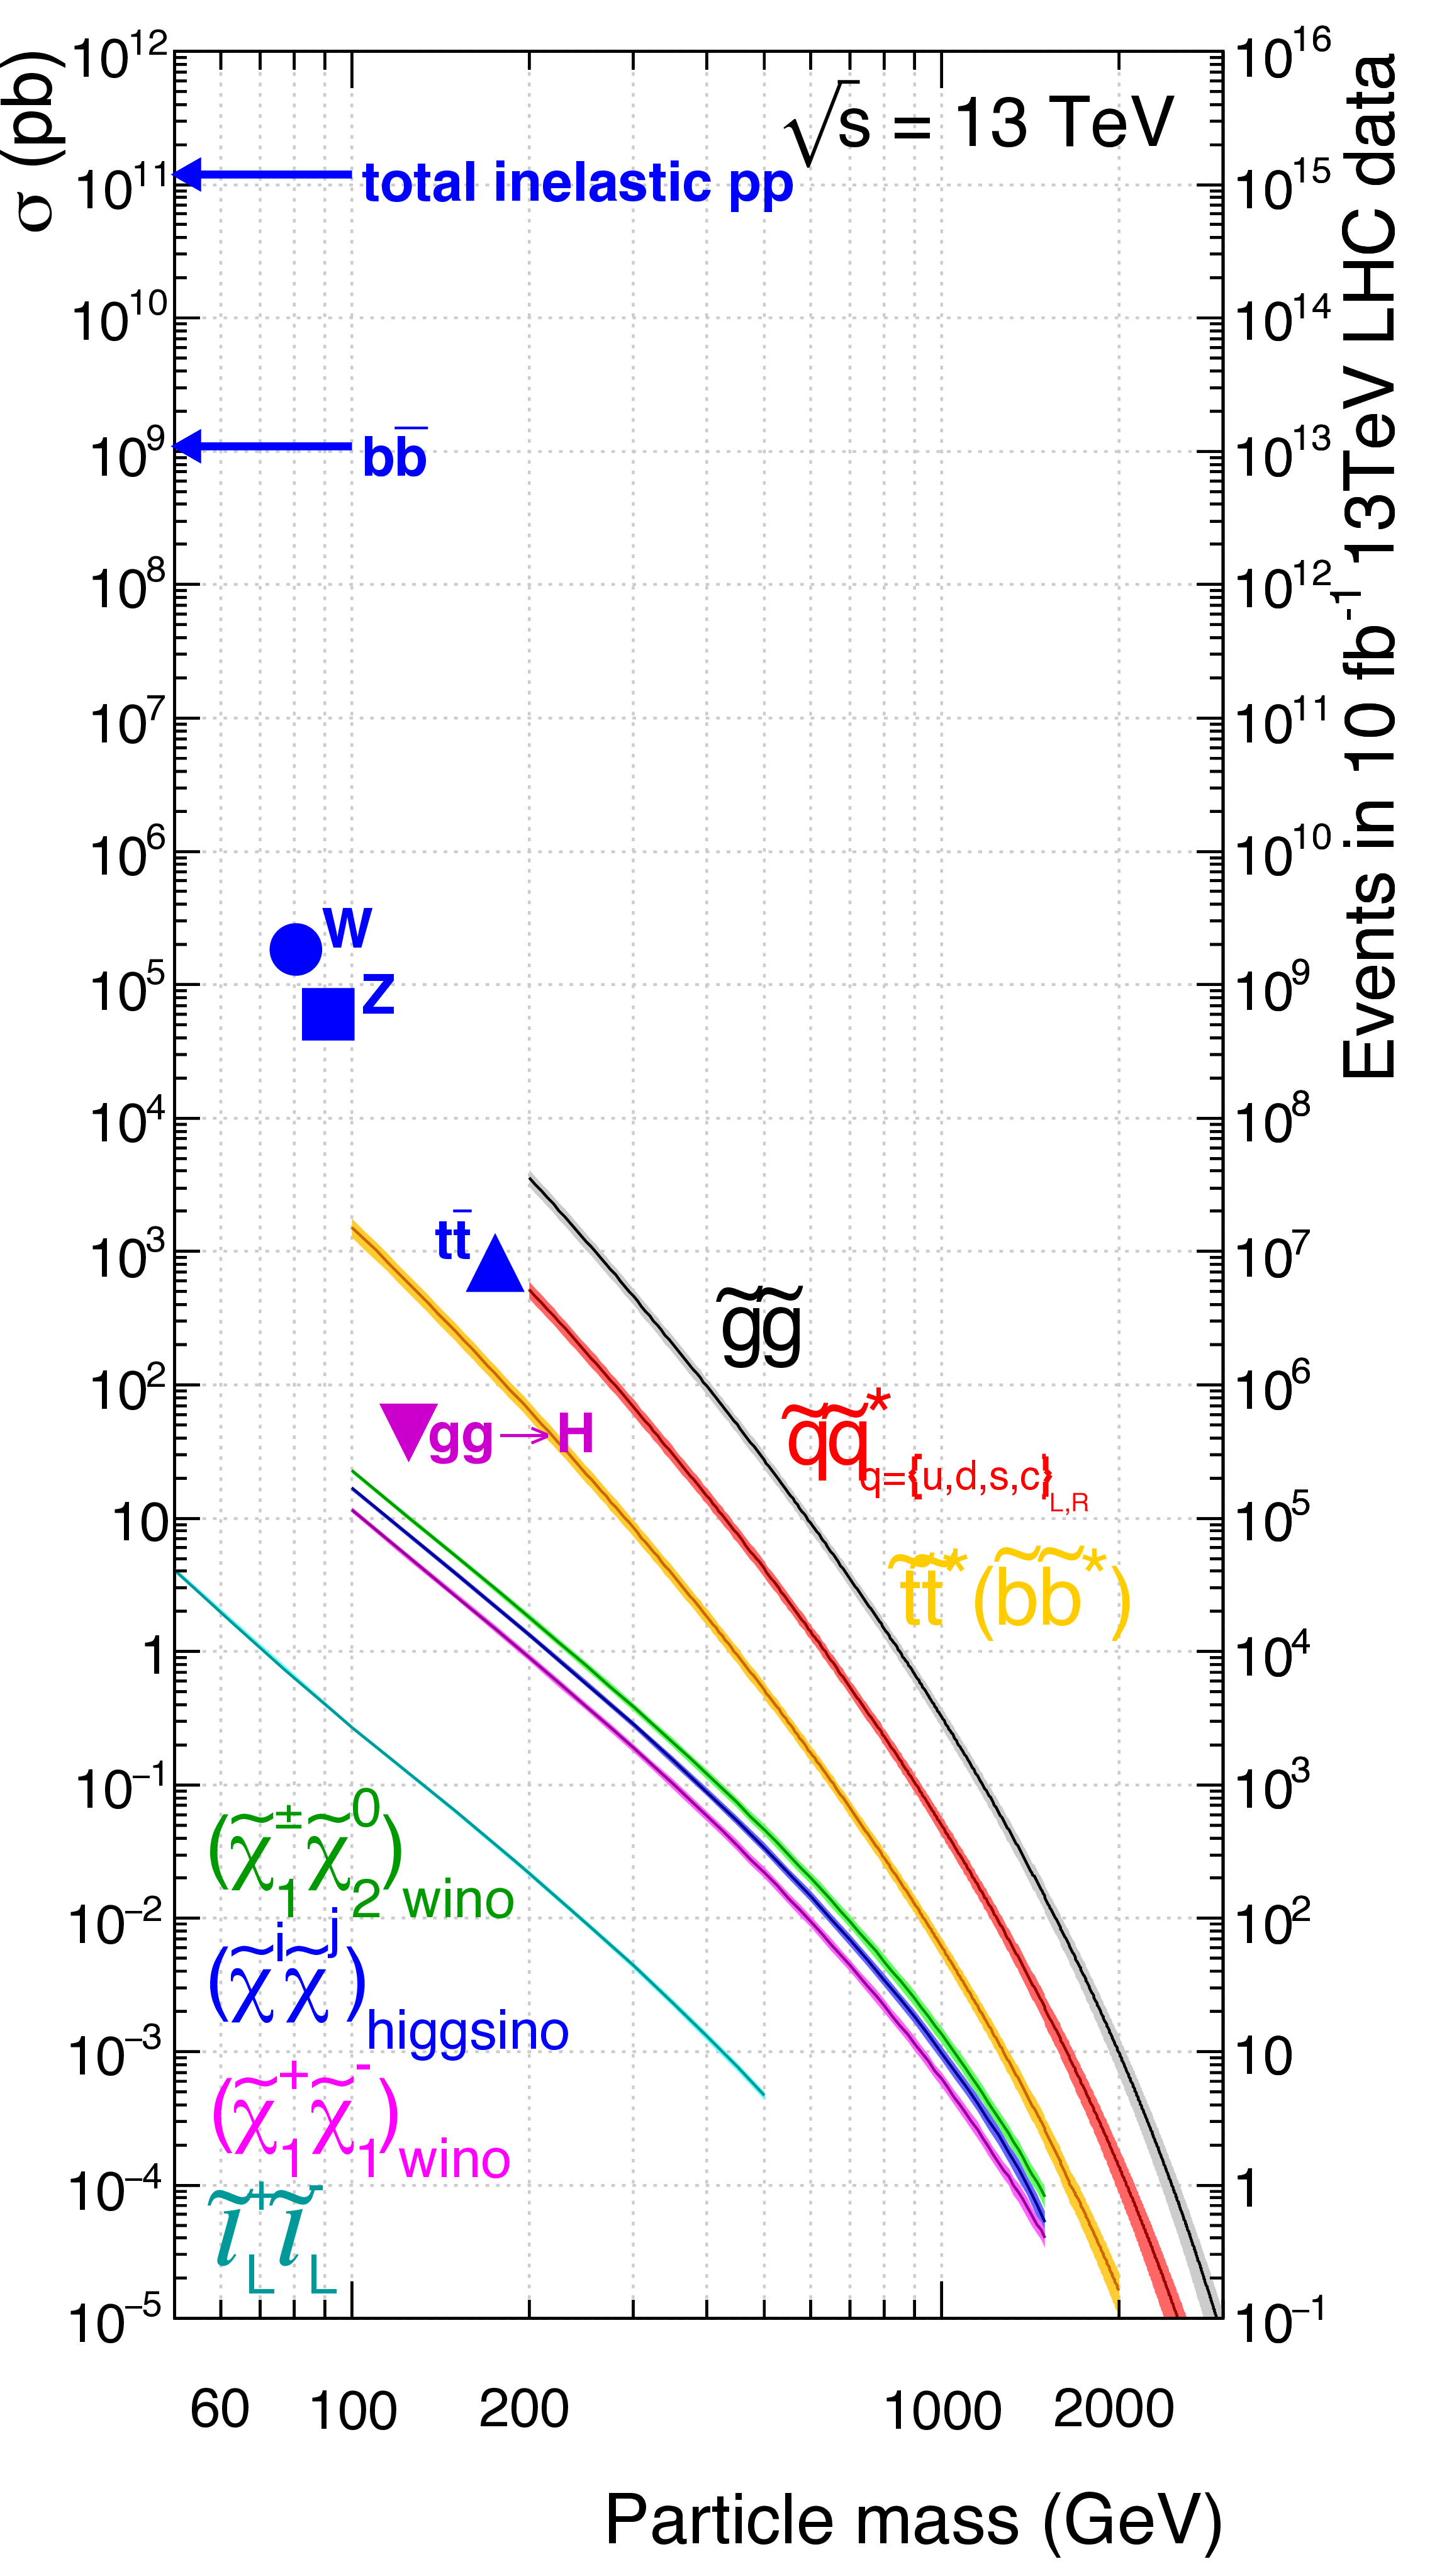
\includegraphics[height=1.25\textwidth]{figs/rpvthreel/xsec10_13_SM.png}
    \caption[Theoretical production cross sections for selected standard model and SUSY in 13\TeV proton collisions. 
    The expected number of events produced for each process in 10~\ifb\ of LHC data is shown on the right scale]{Theoretical production cross sections for selected standard model and SUSY in 13\TeV proton collisions. 
    The expected number of events produced for each process in 10~\ifb\ of LHC data is shown on the right scale~\cite{Borschensky:2014cia}.}
    \label{fig:xsec}
\end{figure}
These are plotted as the green points in Figure \ref{fig:statthrows}.
Running the Renormilization Group (RG) equations down to the EW scale, one finds that of these 4,351,809 appropriate \BL initial points, only 3,142,657 break electroweak symmetry with the experimentally measured values for $M_{Z}$ and $M_{W}$ given in equation.
These are shown as the purple points in Figure~\ref{fig:statthrows}.
Now applying the constraints that all sparticle masses be at or above their currently measured lower bounds~\cite{Dumitru:2018jyb}, it was found that of these 3,142,657 initial points, only 342,236 are acceptable.
These are indicated by cyan colored points in Figure~\ref{fig:statthrows}.
Finally, of these 342,236 points, only 67,576 also lead to the currently measured Higgs mass.
That is, of the 100 million sets of randomly scattered initial conditions, 67,576 satisfy all present phenomenological requirements.
These are referred to as the ``valid" points.
%Whereby "valid" points are those throws that satisfy all current phenomenological bounds. 
As discussed in detail in \cite{Ovrut:2015uea}, the particle spectrum of each of the 67,576 valid black points is exactly determined by the computer code.

The identify of the lighest supersymmetric particle (LSP) in the particle spectrum is particularly interesting when designing experimental searches.
The identity of the LSP is shown in Figure~\ref{fig:LSPprob} in terms of the number and percentage of the valid points that have that type of supersymmetric particle as the LSP.
With the above assumptions for the model and constraints, we now have an effective probability for a given sparticle to be the LSP, a very interesting and useful result.
There are of course experimental considerations to be made when analyzing this histogram that will in general re-weight one's search motivations from Figure \ref{fig:LSPprob} for a given process. 
First is the relative production cross section of each sparticle at the LHC.
Figure \ref{fig:xsec} shows us the production cross sections as a function of mass for various standard model and supersymmetric particles.
The mostly bino-like neutralino ($\tilde{\chi}^{0}_{B}$) is the most probable LSP.
However, if it is pure bino then it cannot be pair-produced directly and so the cross section is not even shown on Figure~\ref{fig:xsec}.

Sneutrinos or sleptons are the LSPs in  about 10\% of the valid model points.
However, experimental searches with Run-2 data are also disfavored as these have a very small production cross section (cyan line in Figure~\ref{fig:xsec}).
These will be left for future searches with more data in Run-3 or HL-LHC.
%\\ \textbf{\textcolor{red}{$\rightarrow$ Say something about sbottoms, gluino, and sup? Covered in other searches maybe? Or just favor ewkinos due to cleaner signals.}}\\
%Bino like neutralinos are not even included due to the smallness of its cross section. 

The mostly wino-like chargino or neutralino are the LSPs in about 10\% of the valid model points.
The experimental production cross sections for wino-type chargino-pair and chargino-neutralino pair production are large enough to allow for a feasible search with Run-2 data (green and magenta lines in Figure~\ref{fig:xsec}).
%\\ \textbf{\textcolor{red}{$\rightarrow$ Would like to have a analogous histogram with the production cross-sections @ 139\ifb for a given sparticle mass, e.g. 1000\gev}}
%\\ \textbf{\textcolor{red}{$\rightarrow$ Want to talk about what types of signals are already well covered}}
%\begin{figure}
%    \centering
%    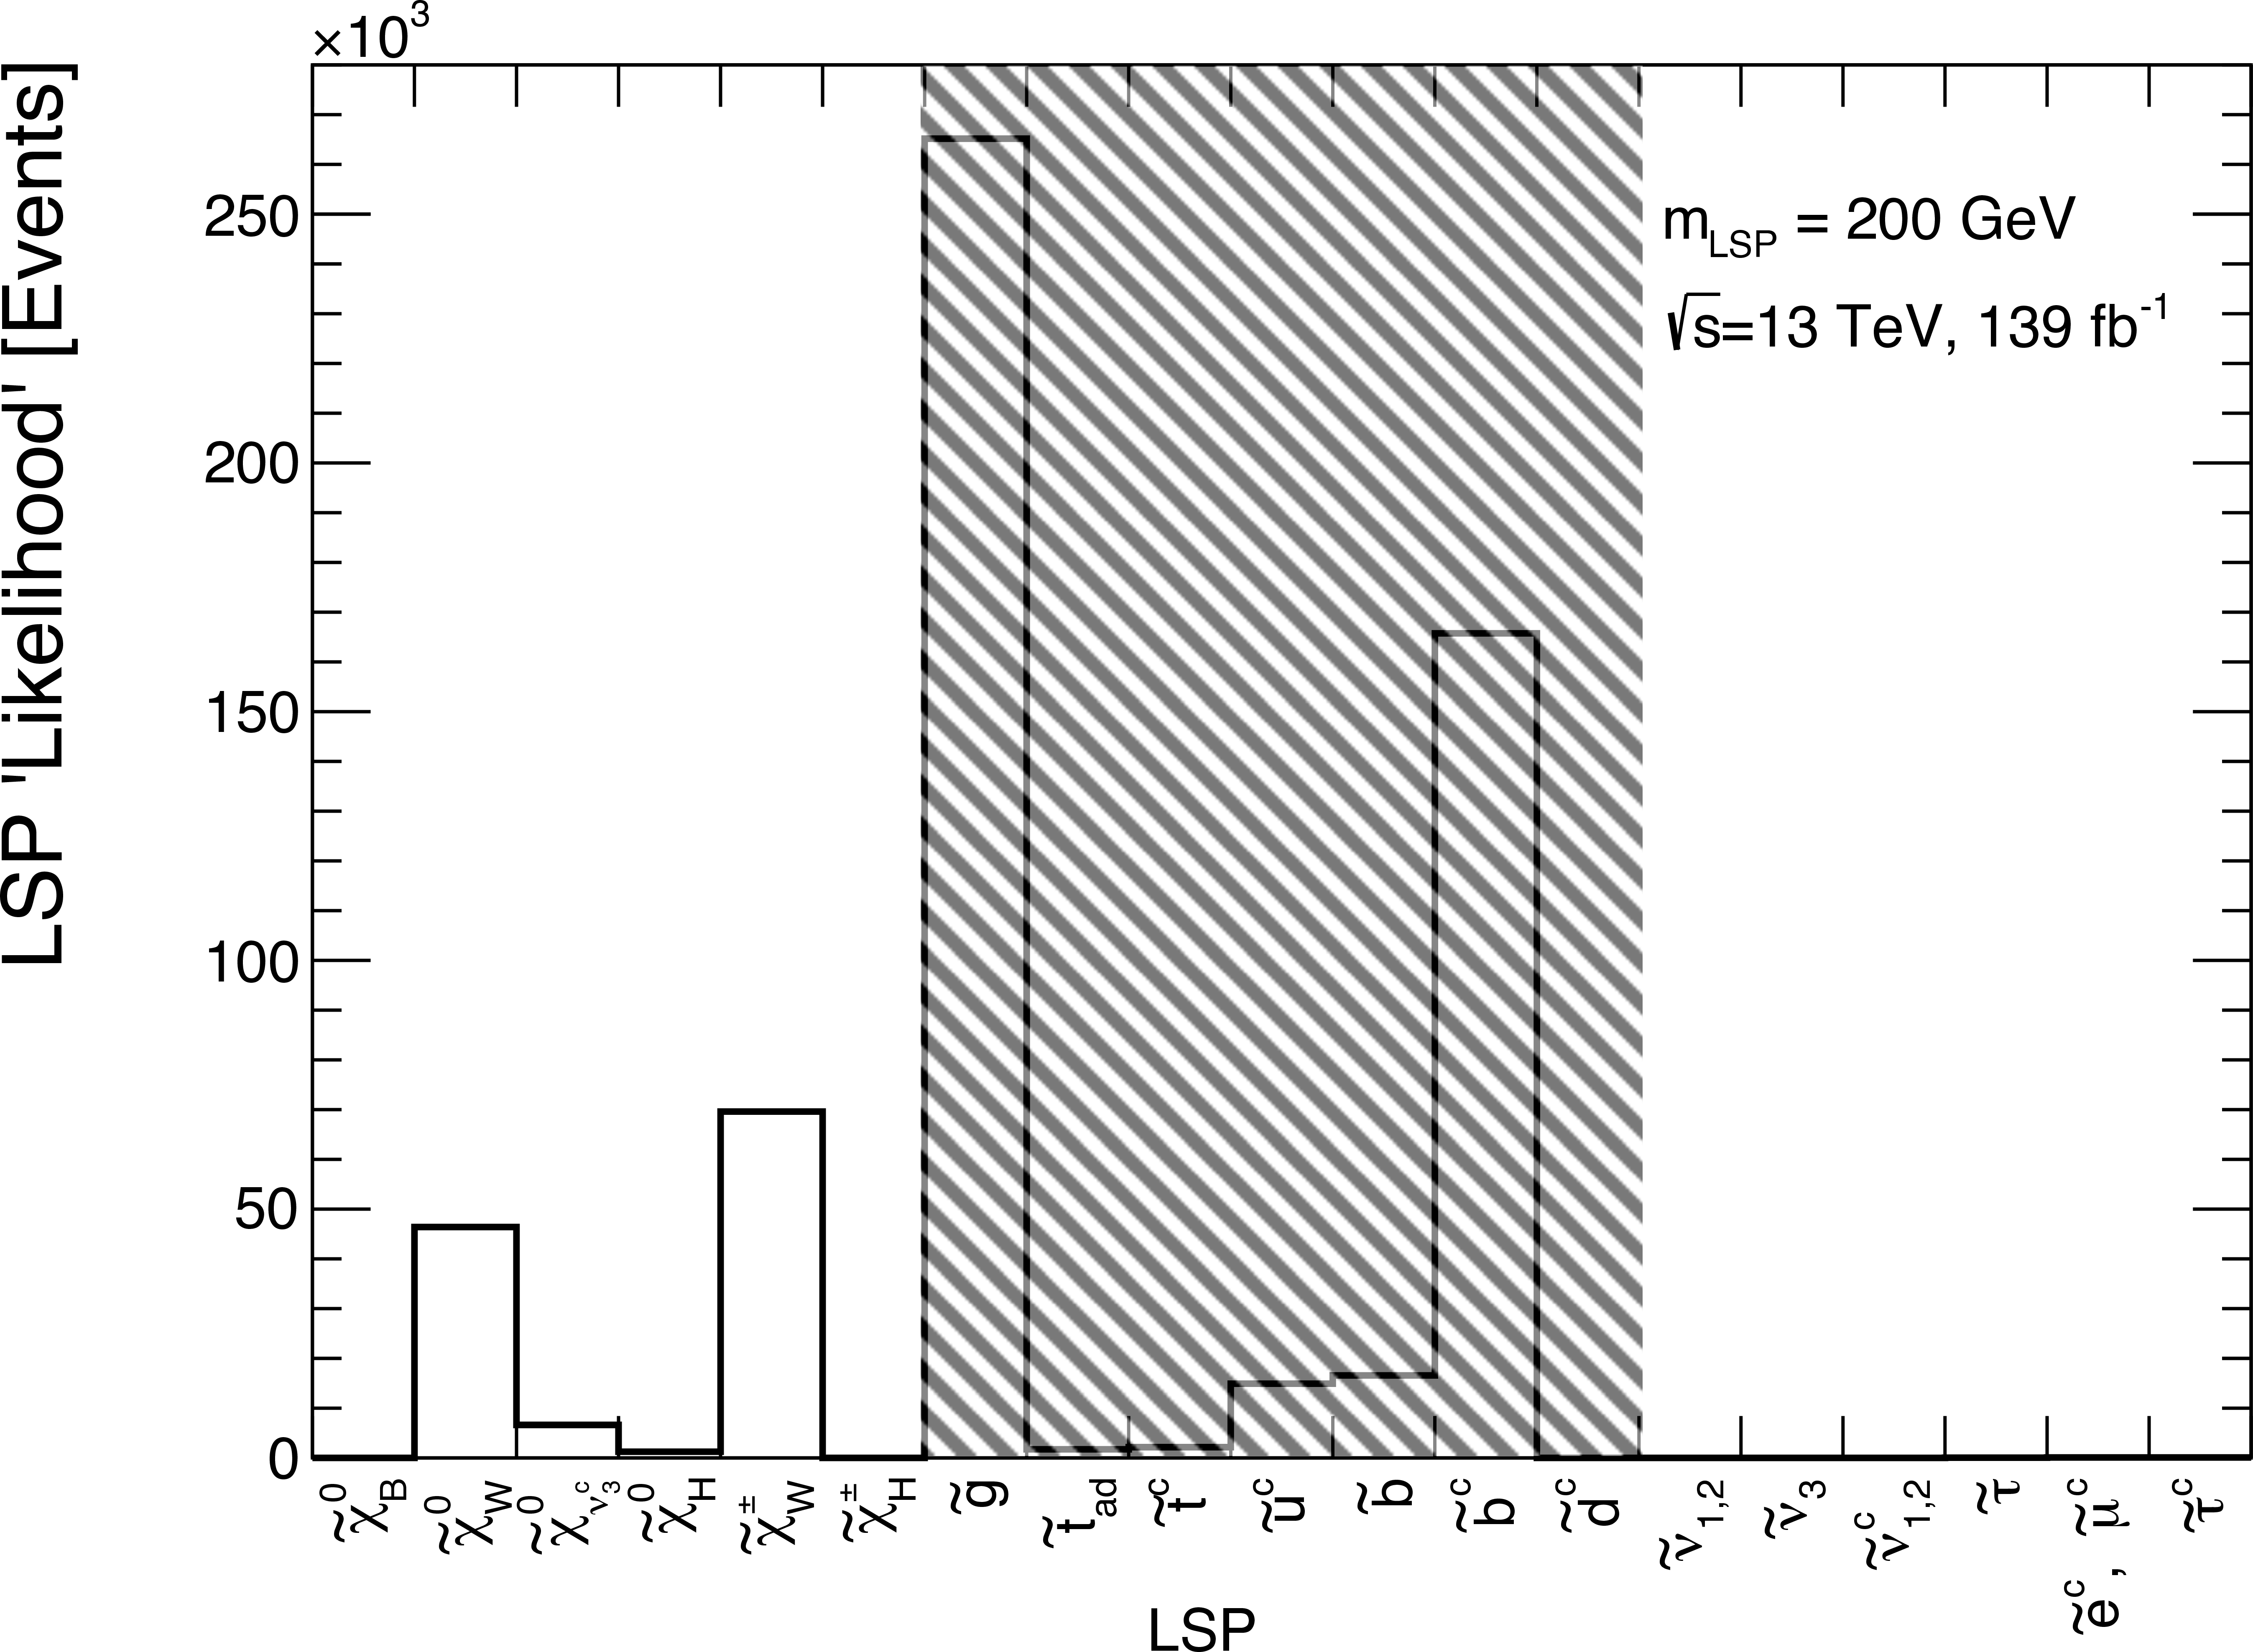
\includegraphics[width=0.95\textwidth]{figs/rpvthreel/LSPprobtimesXS.pdf}
%    \caption[A histogram of the number of sparticles potentially produced in 139\ifb of LHC \rts =13 \tev data reweighted by the likelihood that the sparticle in the LSP]{A histogram of the number of sparticles potentially produced in 139\ifb of LHC \rts =13 \tev data reweighted by the likelihood that the sparticle in the LSP.
%    Electroweak SUSY is only considered for this search, strong SUSY processes appear in middle the hatched section of the histogram.}
%    \label{fig:LSPLikelihood}
%\end{figure}
Due to the relative smallness of the RPV coupling we expect the most probable RPV decays to be from the LSP, however if there is effective mass degeneracy between the LSP and NLSP (a very small mass splitting), it is very reasonable to expect both the LSP and NLSP to both decay via RPV, i.e. all final states will be SM particles only. 
In Figure~\ref{fig:massdeg} where the mass values for the \chono\ are for valid points in the scan in which the \none and \chonemp are either the LSP or NLSP we see mass splittings less than a \gev for cases where the \none is the LSP and \chonepm the NLSP \ref{fig:massdega} and vice versa \ref{fig:massdegb}.
This shows the possibility of a search with sizable production cross sections from the sum of chargino-pair production and mass-degenerate chargino-neutralino production.  Further, both the LSP and NLSP will have RPV decays due to the small size of their mass splitting.
This will be the topic of the search described in this thesis.
\begin{figure}
    \centering
    \begin{subfigure}[b]{0.49\textwidth}
      \centering
      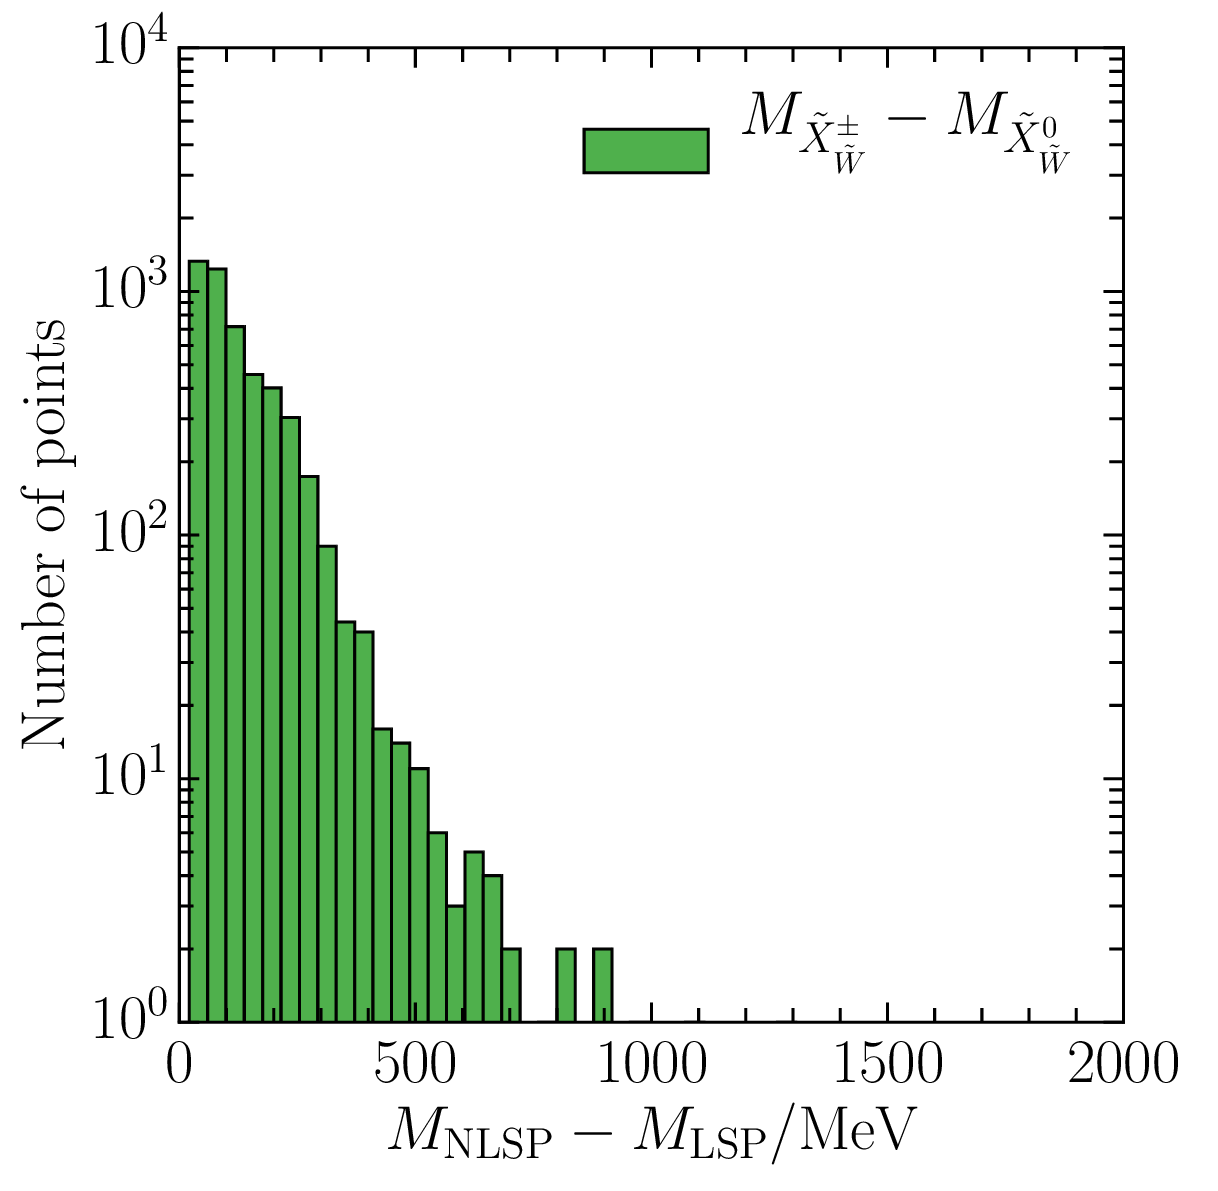
\includegraphics[width=0.98\textwidth]{figs/rpvthreel/MassDegenerateChipm.png}
      \caption{}
      \label{fig:massdega}
    \end{subfigure}
    \hfill
    \begin{subfigure}[b]{0.49\textwidth}
      \centering
      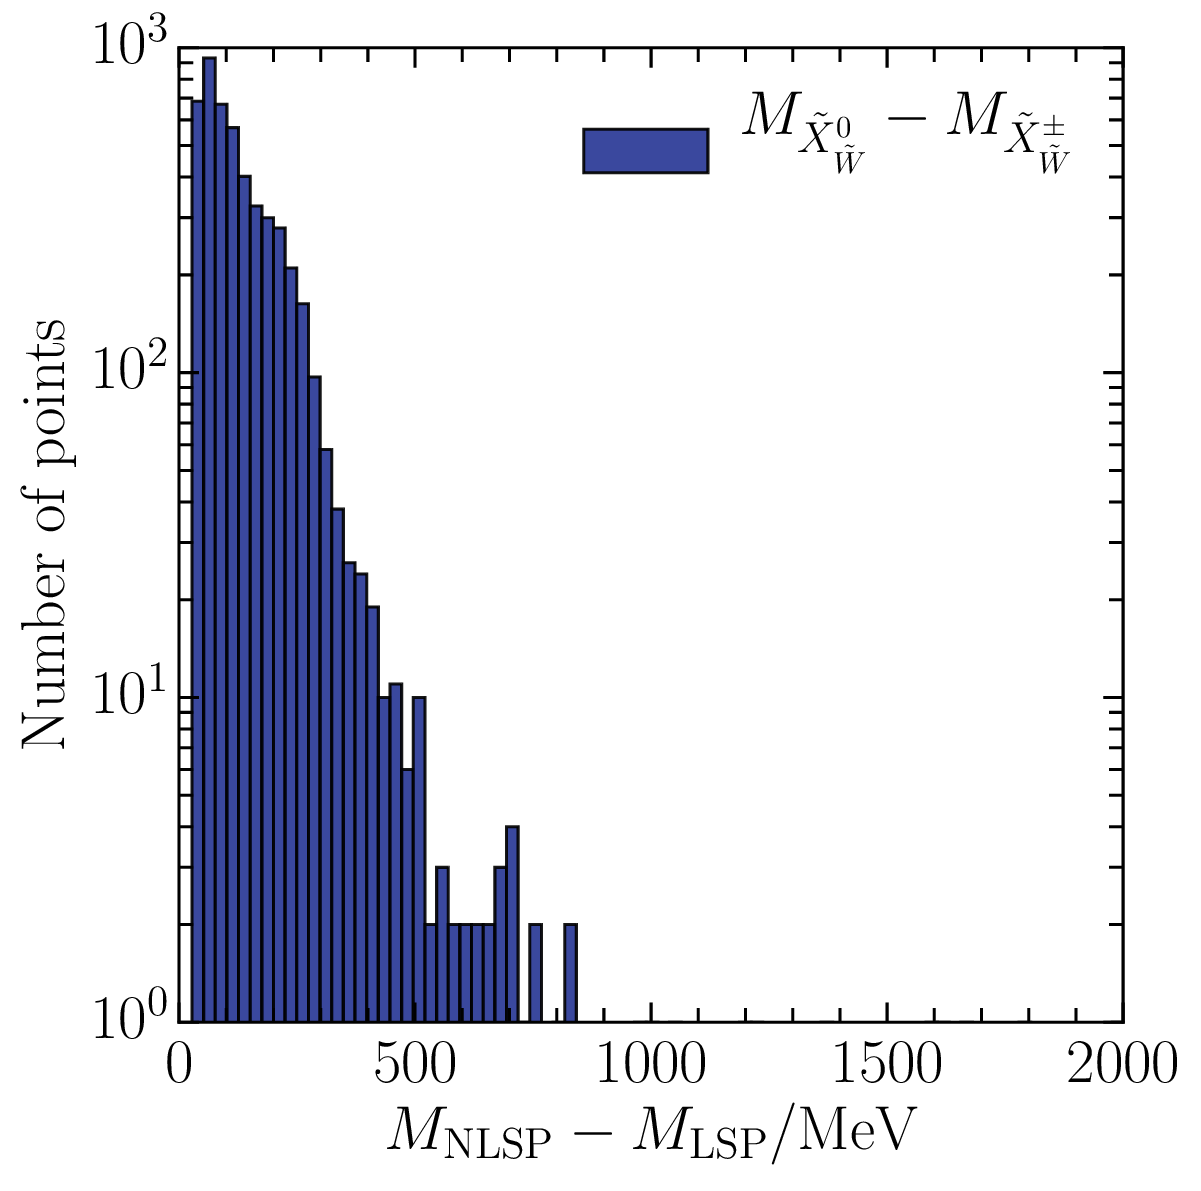
\includegraphics[width=0.98\textwidth]{figs/rpvthreel/MassDegenerateChi0.png}
      \caption{}
      \label{fig:massdegb}
    \end{subfigure}
    \caption[The mass difference between the \chonepm and \none when the \none is the LSP and the \chonepm the NLSP (a) and then again with the \chonepm the LSP and the \none the NLSP (b)]{The mass difference between the \chonepm and \none when the \none is the LSP and the \chonepm the NLSP (a) and then again with the \chonepm the LSP and the \none the NLSP (b) \cite{Dumitru:2018nct}.}
    \label{fig:massdeg}
\end{figure}
The remaining LSPs have a low probability but would be produced profusely through strong production processes.
An earlier analysis by my adviser's group searched for pair production of a stop LSP with RPV decay~\cite{ATLAS:2017jvy} in early Run-2 data.


%
%\begin{figure}
%    \centering
%    \begin{subfigure}[b]{0.49\textwidth}
%      \centering
%      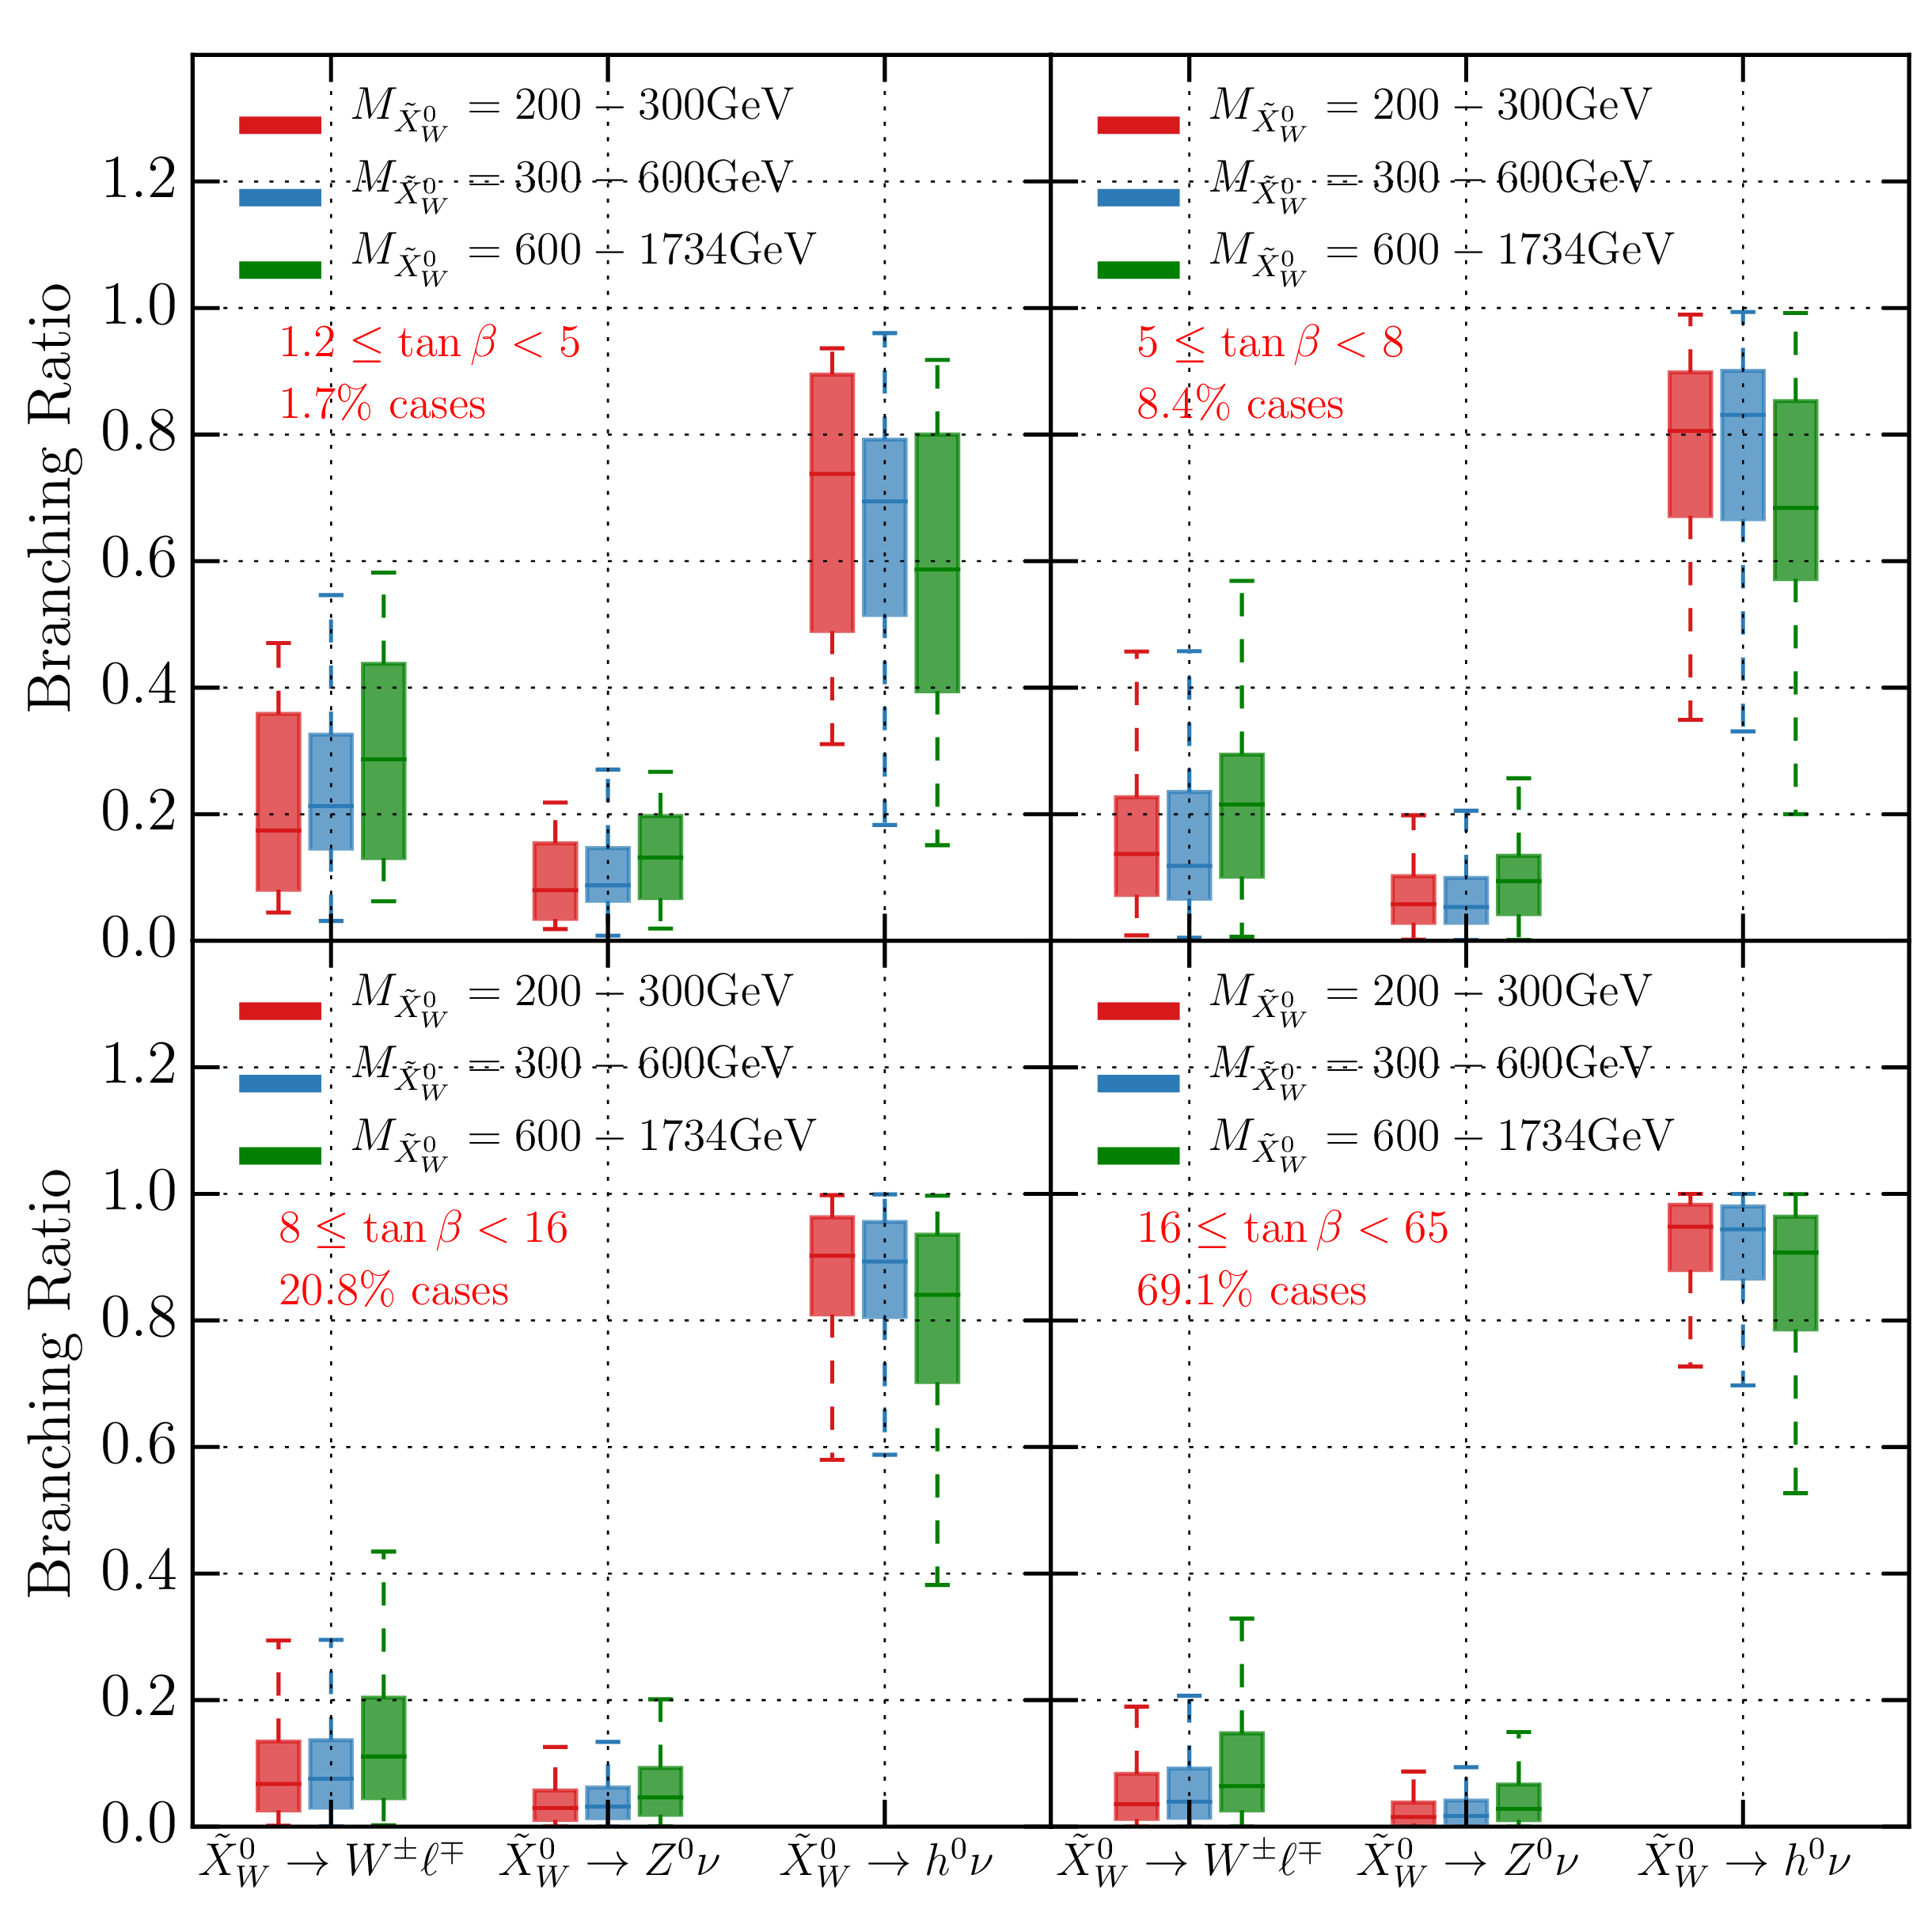
\includegraphics[width=0.98\textwidth]{figs/rpvthreel/TheoryBRsChi0LSP.pdf}
%      \caption{}
%      \label{fig:massdega}
%    \end{subfigure}
%    \hfill
%    \begin{subfigure}[b]{0.49\textwidth}
%      \centering
%      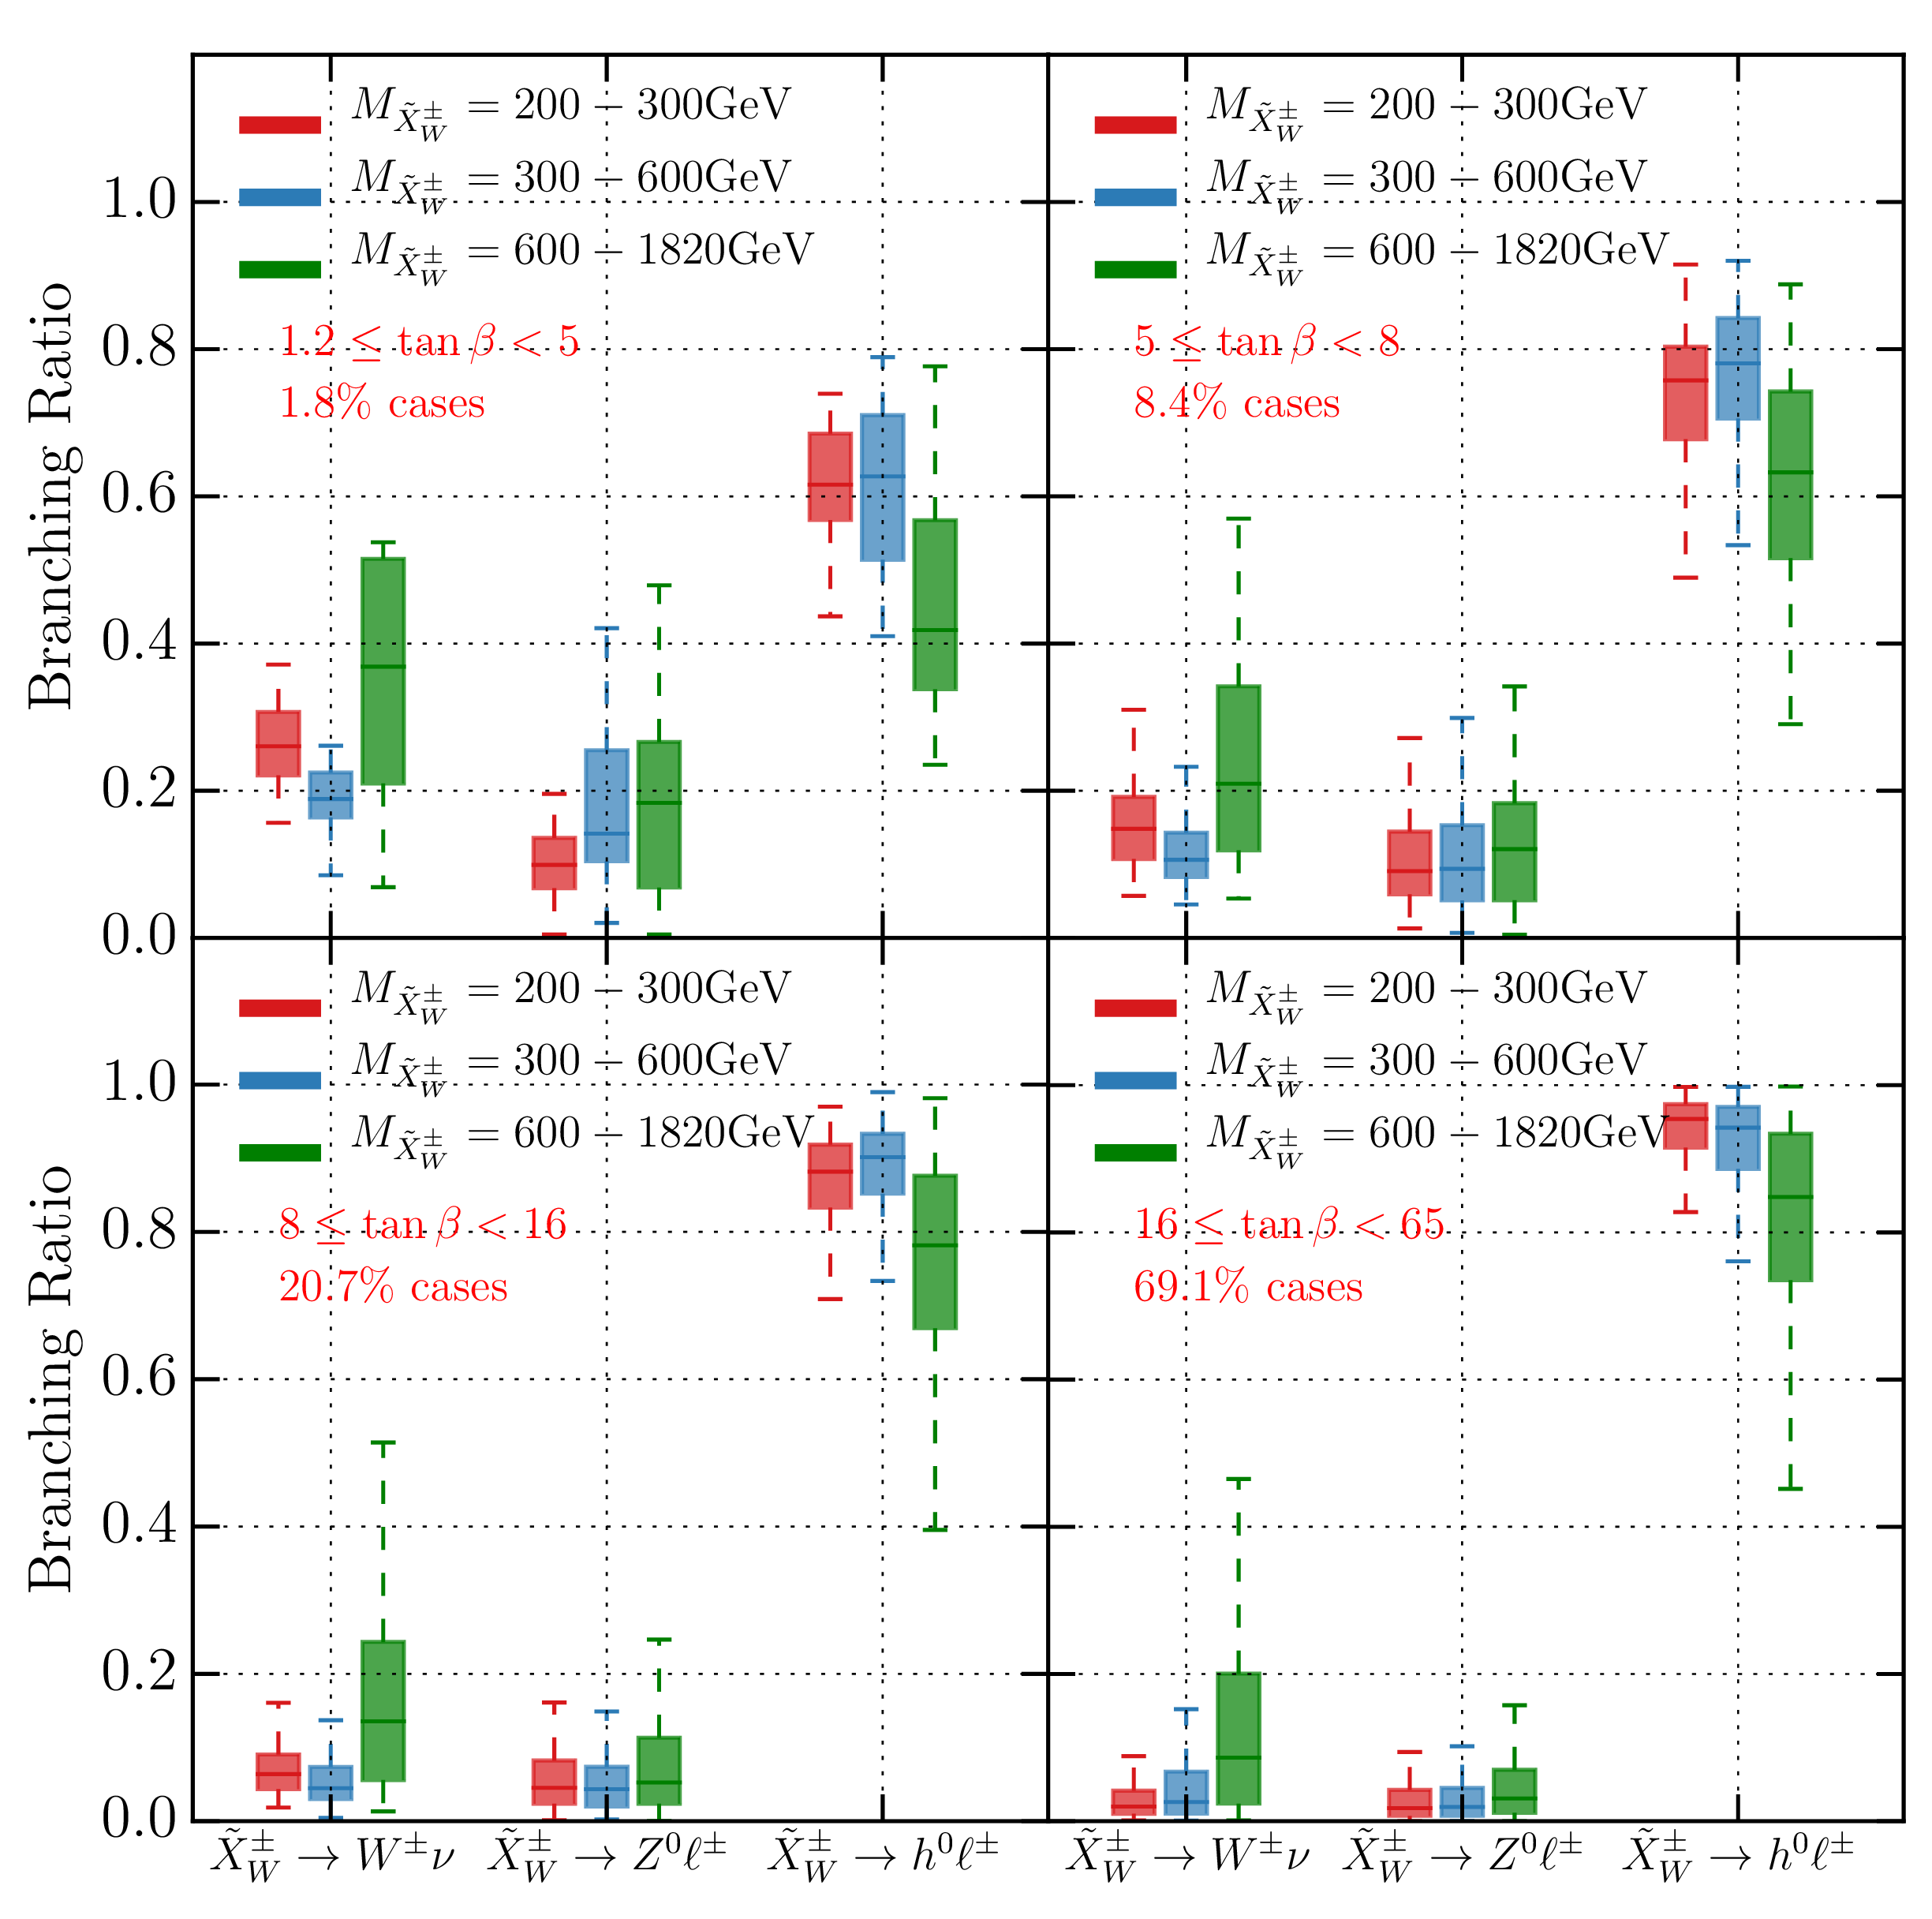
\includegraphics[width=0.98\textwidth]{figs/rpvthreel/TheoryBRsChipmLSP.pdf}
%      \caption{}
%      \label{fig:massdegb}
%    \end{subfigure}
%    \caption[]{Caption \cite{Dumitru:2018nct}}
%    \label{fig:massdeg}
%\end{figure}
